% !TEX program = xelatex
% com_ideal_v6_dither_analysis.tex
% COM_ideal V6 理想锁存比较器：校准专用确定性 sub-LSB 阈值抖动机制分析
\documentclass[UTF8,a4paper,11pt]{ctexart}

% ==================== 页面 ====================
\usepackage[margin=2.25cm]{geometry}

% ==================== 数学 ====================
\usepackage{amsmath}
\usepackage{amssymb}
\usepackage{mathtools}
\usepackage{bm}

% ==================== 表格 ====================
\usepackage{booktabs}
\usepackage{array}
\usepackage{tabularx}
\usepackage{longtable}
\usepackage{multirow}
\usepackage{makecell}

% ==================== 图形 ====================
\usepackage{graphicx}
\usepackage{float}
\usepackage{caption}
\usepackage{subcaption}

% ==================== TikZ ====================
\usepackage{tikz}
\usetikzlibrary{
  arrows.meta,
  positioning,
  shapes.geometric,
  fit,
  calc,
  backgrounds,
  decorations.pathreplacing
}

% ==================== 列表 ====================
\usepackage{enumitem}

% ==================== 代码 ====================
\usepackage{listings}

% ==================== 算法 ====================
\usepackage{algorithm}
\usepackage{algpseudocode}

% ==================== 排版微调 ====================
\usepackage{microtype}

% ==================== 颜色和链接 ====================
\usepackage{xcolor}
\usepackage{hyperref}
\usepackage[nameinlink,noabbrev]{cleveref}

% ==================== tcolorbox ====================
\usepackage{tcolorbox}
\tcbuselibrary{skins,breakable}

% ==================== 颜色体系 ====================
\definecolor{navy}{HTML}{163A5F}
\definecolor{teal}{HTML}{167C80}
\definecolor{orange}{HTML}{D97706}
\definecolor{redx}{HTML}{B42318}
\definecolor{lightblue}{HTML}{EAF2F8}
\definecolor{lightteal}{HTML}{E8F5F4}
\definecolor{lightorange}{HTML}{FFF3E0}
\definecolor{graybox}{HTML}{F3F4F6}

% tcolorbox 提示框颜色（第一版方案）
\definecolor{tipblue}{RGB}{220,235,250}
\definecolor{tipblueframe}{RGB}{60,100,180}
\definecolor{warnyellow}{RGB}{255,248,220}
\definecolor{warnyellowframe}{RGB}{200,150,30}
\definecolor{keygreeng}{RGB}{225,245,225}
\definecolor{keygreengframe}{RGB}{40,140,60}
\definecolor{notegray}{RGB}{240,240,240}
\definecolor{notegrayframe}{RGB}{120,120,120}

\hypersetup{
  colorlinks=true,
  linkcolor=navy,
  citecolor=teal,
  urlcolor=navy,
  pdftitle={COM_ideal V6 比较器抖动机制分析},
  pdfauthor={混合信号IC设计技术文档}
}

% ==================== 列表与表格间距 ====================
\setlist[itemize]{
  leftmargin=2em,
  itemsep=0.25em,
  topsep=0.35em
}
\setlist[enumerate]{
  leftmargin=2.2em,
  itemsep=0.3em,
  topsep=0.35em
}
\renewcommand{\arraystretch}{1.25}

\captionsetup{
  font=small,
  labelfont=bf
}

% ==================== 代码风格 ====================
\lstset{
  basicstyle=\ttfamily\small,
  backgroundcolor=\color{graybox},
  frame=single,
  rulecolor=\color{gray!35},
  breaklines=true,
  columns=fullflexible,
  showstringspaces=false,
  keywordstyle=\color{navy}\bfseries,
  commentstyle=\color{teal},
  numbers=left,
  numberstyle=\tiny\color{gray},
  xleftmargin=1.5em,
  framexleftmargin=1.2em,
  language=Verilog
}

% ==================== 算法伪代码汉化 ====================
\renewcommand{\algorithmicrequire}{\textbf{输入:}}
\renewcommand{\algorithmicensure}{\textbf{输出:}}
\renewcommand{\algorithmicif}{\textbf{若}}
\renewcommand{\algorithmicthen}{\textbf{则}}
\renewcommand{\algorithmicelse}{\textbf{否则}}
\renewcommand{\algorithmicfor}{\textbf{对于}}
\renewcommand{\algorithmicdo}{\textbf{执行}}
\renewcommand{\algorithmicwhile}{\textbf{当}}
\renewcommand{\algorithmicreturn}{\textbf{返回}}
\renewcommand{\algorithmicprocedure}{\textbf{过程}}
\renewcommand{\algorithmicend}{\textbf{结束}}

% ==================== tcolorbox 提示框环境 ====================
\newtcolorbox{tipbox}[1]{%
  enhanced, breakable,
  colback=tipblue, colframe=tipblueframe,
  boxrule=0.5pt, arc=2pt,
  left=8pt, right=8pt, top=6pt, bottom=6pt,
  fonttitle=\bfseries\small,
  title={#1}
}

\newtcolorbox{warnbox}[1]{%
  enhanced, breakable,
  colback=warnyellow, colframe=warnyellowframe,
  boxrule=0.5pt, arc=2pt,
  left=8pt, right=8pt, top=6pt, bottom=6pt,
  fonttitle=\bfseries\small,
  title={#1}
}

\newtcolorbox{keybox}[1]{%
  enhanced, breakable,
  colback=keygreeng, colframe=keygreengframe,
  boxrule=0.5pt, arc=2pt,
  left=8pt, right=8pt, top=6pt, bottom=6pt,
  fonttitle=\bfseries\small,
  title={#1}
}

\newtcolorbox{notebox}[1]{%
  enhanced, breakable,
  colback=notegray, colframe=notegrayframe,
  boxrule=0.5pt, arc=2pt,
  left=8pt, right=8pt, top=6pt, bottom=6pt,
  fonttitle=\bfseries\small,
  title={#1}
}

% ==================== 便捷命令 ====================
\newcommand{\Vref}{V_{\mathrm{REF}}}
\newcommand{\Vcal}{V_{\mathrm{cal}}}
\newcommand{\Vlsb}{V_{\mathrm{LSB,cal}}}
\newcommand{\Vdith}{V_{\mathrm{dith}}}
\newcommand{\vdiff}{v_{\mathrm{diff}}}
\newcommand{\dith}{d}
\newcommand{\code}[1]{\texttt{#1}}

% ==================== TikZ 节点风格 ====================
\tikzset{
  block/.style={
    rectangle,
    rounded corners,
    draw=navy,
    thick,
    fill=lightblue,
    align=center,
    minimum height=9mm,
    text width=32mm,
    inner sep=4pt
  },
  smallblock/.style={
    rectangle,
    rounded corners,
    draw=teal,
    thick,
    fill=lightteal,
    align=center,
    minimum height=7mm,
    text width=24mm,
    inner sep=3pt
  },
  decision/.style={
    diamond,
    draw=teal,
    thick,
    fill=lightteal,
    align=center,
    aspect=2,
    inner sep=2pt
  },
  arrow/.style={
    -{Stealth[length=2.2mm]},
    thick,
    draw=navy
  },
  darrow/.style={
    -{Stealth[length=2.2mm]},
    thick,
    draw=teal,
    dashed
  }
}

% ==================== 文档信息 ====================
\title{\textbf{COM\_ideal V6 理想锁存比较器：\\[4pt]
校准专用确定性 sub-LSB 阈值抖动机制分析}}
\author{混合信号 IC 设计技术文档}
\date{2026年7月}

\begin{document}

\maketitle

% ==================== 摘要 ====================
\begin{abstract}
\noindent
本文系统分析 \code{COM\_ideal} V6 Verilog-A 行为级比较器模型的核心设计：\textbf{校准专用确定性 sub-LSB 阈值抖动}（deterministic sub-LSB threshold dither）。该机制在校准模式（\code{CAL=1}）下，将比较器判决阈值在一个校准 LSB 区间内按 32 个中点均匀步进扫描，使校准引擎能够在 calDAC 离散步长（4 LSB）之上获得 sub-LSB 测量分辨率；在正常转换模式（\code{CAL=0}）下抖动严格为零，保证 bypass 测试和校准后 A/B 验证的纯净性。文章推导了抖动电压公式 $V_{\mathrm{dith},k} = \Vlsb \cdot \frac{k+0.5}{N} - \frac{\Vlsb}{2}$、时序状态机（16 edge/pair、32 level/sequence）、以及 sub-LSB 编码原理，并通过数值例子验证其自洽性。
\end{abstract}

\bigskip

\tableofcontents
\newpage

% ==================== 1. 概述 ====================
\section{概述}

\code{COM\_ideal} V6 是一个理想锁存差分比较器的 Verilog-A 行为级模型，专为 12 位非二进制冗余 SAR ADC 的前景权重校准而设计。其核心创新在于：\textbf{仅在校准模式下注入确定性的 sub-LSB 阈值抖动}，从而让校准引擎能够测量小于一个 calDAC 步长的残差。

\begin{tipbox}{设计目标}
比较器的物理功能只有一件事：判断 $V_P > V_N$ 还是 $V_P < V_N$，并输出差分逻辑电平。V6 的全部复杂性都集中在\textbf{校准模式下的阈值抖动注入}——这不是比较器本身的需求，而是校准引擎对 sub-LSB 分辨率的需求。
\end{tipbox}

该模块的关键特性概括如下：

\begin{itemize}[leftmargin=2em]
    \item \textbf{理想比较器}：零延迟（除 TD=20ps 外）、零噪声、可选失调 \code{VOS}；
    \item \textbf{校准专用抖动}：仅在 \code{CAL=1} 时注入，\code{CAL=0} 时严格为零；
    \item \textbf{确定性扫描}：32 个中点均匀步进，覆盖 $[-0.5, +0.5)$ 校准 LSB；
    \item \textbf{成对保持}：每个 D+/D$-$ 对（16 个 CLK 边沿）使用同一抖动值；
    \item \textbf{有限 R 驱动}：输出用 \code{RDRV=1$\Omega$} 避免刚性支路环路。
\end{itemize}

% ==================== 2. 模块接口与参数 ====================
\section{模块接口与参数}

\subsection{端口定义}

模块采用固定位置参数接口，与 SAR ADC 顶层网表直接对接：

\begin{table}[H]
\centering
\caption{COM\_ideal V6 端口定义}
\label{tab:ports}
\small
\begin{tabularx}{\textwidth}{l l l X}
\toprule
端口 & 方向 & 类型 & 说明 \\
\midrule
\code{CLK} & input & electrical & 比较器时钟（锁存触发沿） \\
\code{P} & input & electrical & 正相输入 \\
\code{N} & input & electrical & 负相输入 \\
\code{CAL} & input & electrical & 校准使能（高有效） \\
\code{COMP} & output & electrical & 正相输出（$P>N$ 时为高） \\
\code{COMN} & output & electrical & 负相输出（$P<N$ 时为高） \\
\bottomrule
\end{tabularx}
\end{table}

\begin{notebox}{极性约定}
$V_P > V_N \Rightarrow \code{COMP}=1, \code{COMN}=0$（正相输出高）；$V_P < V_N \Rightarrow \code{COMP}=0, \code{COMN}=1$。差分输出严格互补，便于 SAR 逻辑直接锁存。
\end{notebox}

\subsection{关键参数}

\begin{table}[H]
\centering
\caption{关键参数一览}
\label{tab:params}
\small
\begin{tabularx}{\textwidth}{l l l X}
\toprule
参数 & 默认值 & 类别 & 说明 \\
\midrule
\code{VHIGH} & 1.8 & 输出 & 输出高电平 \\
\code{VTH\_CLK} & 0.9 & 时钟 & CLK 判决阈值 \\
\code{VTH\_CAL} & 0.9 & 校准 & CAL 判决阈值 \\
\code{VOS} & 0.0 & 失调 & 输入等效失调电压 \\
\code{TD/TR/TF} & 20p/10p/10p & 时序 & 输出延迟与转换时间 \\
\code{RDRV} & 1.0 & 驱动 & 输出驱动电阻（$\Omega$） \\
\code{TIE\_P\_GT\_N} & 0 & 判决 & $V_P = V_N$ 时的输出极性 \\
\code{CAL\_DITHER\_ENABLE} & 1 & 抖动 & 校准抖动总使能 \\
\code{CAL\_LSB\_V} & 0.8274m & 抖动 & 一个校准码 LSB 对应的差分电压 \\
\code{DITHER\_LEVELS} & 32 & 抖动 & 抖动序列长度 \\
\code{DITHER\_PAIR\_EDGES} & 16 & 抖动 & 每个 D+/D$-$ 对的 CLK 边沿数 \\
\bottomrule
\end{tabularx}
\end{table}

\begin{keybox}{CAL\_LSB\_V 的物理来源}
$\Vlsb = 0.8274\,\mathrm{mV}$ 来自 SAR ADC 的全量程设计：
\begin{equation}
\Vlsb = \frac{2 \times (V_{\mathrm{REFP}} - V_{\mathrm{REFN}})}{W_{\mathrm{total}}} = \frac{2 \times 1.8}{4351} = 0.8274\,\mathrm{mV}
\end{equation}
其中 $W_{\mathrm{total}} = 4351$ 是 14 个非二进制冗余权重之和，$2 \times 1.8\,\mathrm{V}$ 是差分满量程。这定义了\textbf{一个校准码 LSB 对应的差分电压}，即 calDAC 改变一个码时 $V_P - V_N$ 的变化量。
\end{keybox}

% ==================== 3. 状态变量与信号流 ====================
\section{状态变量与信号流}

\subsection{状态变量}

模块使用四个整数/实数状态变量维护抖动状态机：

\begin{table}[H]
\centering
\caption{状态变量}
\label{tab:statevars}
\small
\begin{tabularx}{\textwidth}{l l X}
\toprule
变量 & 类型 & 功能 \\
\midrule
\code{comp\_state\_i} & integer & 比较器输出状态（0 或 1） \\
\code{edge\_in\_pair\_i} & integer & 当前 D+/D$-$ 对内的 CLK 边沿计数（0$\sim$15） \\
\code{dither\_index\_i} & integer & 抖动序列索引（0$\sim$31） \\
\code{dither\_v\_i} & real & 当前抖动电压值 \\
\code{vdiff\_i} & real & 有效差分输入（含失调和抖动） \\
\code{cal\_i} & integer & CAL 信号的数字采样值 \\
\bottomrule
\end{tabularx}
\end{table}

\subsection{信号流图}

比较器的信号流如\cref{fig:signalflow}所示。

\begin{figure}[H]
\centering
\begin{tikzpicture}[node distance=1.2cm and 1.5cm]
\node[block] (input) {差分输入\\$V_P, V_N$};
\node[block, right=of input] (sub) {减法器\\$V(P,N) - \code{VOS}$};
\node[block, right=of sub] (dith) {减抖动\\$- \Vdith$};
\node[block, right=of dith] (dec) {判决\\$\vdiff > 0 ?$};
\node[block, below=1.5cm of dith] (state) {抖动\\状态机};
\node[block, left=of state] (cal) {CAL\\边沿检测};

\draw[arrow] (input) -- (sub);
\draw[arrow] (sub) -- (dith);
\draw[arrow] (dith) -- (dec);
\draw[darrow] (cal) -- (state);
\draw[darrow] (state) -- (dith);
\draw[arrow] (dec) -- ++(2.5,0) node[right]{$\code{comp\_state\_i}$};
\end{tikzpicture}
\caption{COM\_ideal V6 信号流：输入差分电压减去失调和抖动后进行符号判决}
\label{fig:signalflow}
\end{figure}

% ==================== 4. CAL 信号处理 ====================
\section{CAL 信号边沿处理}

模块对 \code{CAL} 信号的上升沿和下降沿分别处理，确保抖动状态机的生命周期与校准会话严格对齐。

\subsection{CAL 上升沿：初始化抖动序列}

\begin{lstlisting}[language=Verilog]
@(cross(V(CAL) - VTH_CAL, +1)) begin
    edge_in_pair_i = 0;
    dither_index_i = 0;
    dither_v_i = CAL_LSB_V *
        ((0.5 / (1.0*DITHER_LEVELS)) - 0.5);
end
\end{lstlisting}

当 \code{CAL} 从低变高时：

\begin{enumerate}[leftmargin=2em]
    \item 边沿计数器清零：\code{edge\_in\_pair\_i = 0}；
    \item 抖动索引清零：\code{dither\_index\_i = 0}；
    \item 抖动电压初始化为第一个中点值：
\end{enumerate}

\begin{equation}
\Vdith^{(0)} = \Vlsb \cdot \left(\frac{0.5}{N} - \frac{1}{2}\right) = \Vlsb \cdot \frac{0.5 - N/2}{N}
\label{eq:dither_init}
\end{equation}

其中 $N = \code{DITHER\_LEVELS} = 32$。代入数值：

\begin{equation}
\Vdith^{(0)} = 0.8274\,\mathrm{mV} \times \left(\frac{0.5}{32} - 0.5\right) = 0.8274 \times (-0.484375) = -0.4007\,\mathrm{mV}
\end{equation}

\begin{tipbox}{为什么用 $0.5/N$ 而不是 $0$？}
这是\textbf{中点法则}（midpoint rule）的核心。如果第一个抖动值取 $k=0$ 对应 $-0.5\,\Vlsb$（区间左端点），那么它只代表 $[-0.5, -0.5+1/N)$ 这一小段的左边界，不能代表整段的平均值。取 $k=0$ 对应中点 $-0.5 + 0.5/N = -0.484375\,\Vlsb$，则它代表 $[-0.5, -0.5+1/N)$ 这一小段的中心，是数值积分中误差最小的取法。
\end{tipbox}

\subsection{CAL 下降沿：清零抖动}

\begin{lstlisting}[language=Verilog]
@(cross(V(CAL) - VTH_CAL, -1)) begin
    edge_in_pair_i = 0;
    dither_index_i = 0;
    dither_v_i = 0.0;
end
\end{lstlisting}

当 \code{CAL} 从高变低时，抖动立即归零。这保证了\textbf{正常转换模式下比较器完全理想}，没有任何随机行为污染 bypass 测试或校准后 A/B 验证。

\begin{warnbox}{关键设计约束}
\code{CAL=0} 时抖动必须严格为零。如果残留任何抖动，校准后 A/B 测试（校准权重 vs 标称权重对比）将无法反映权重的真实改善，因为抖动本身会引入额外的码值分散。
\end{warnbox}

% ==================== 5. 抖动公式推导（核心） ====================
\section{抖动公式推导（核心）}

\subsection{原始公式}

在每个 D+/D$-$ 对的开始（\code{edge\_in\_pair\_i == 0}），抖动电压按以下公式更新：

\begin{equation}
\boxed{
V_{\mathrm{dith},k} = \Vlsb \cdot \left(\frac{k + 0.5}{N} - \frac{1}{2}\right), \quad k = 0, 1, \ldots, N-1
}
\label{eq:dither_formula}
\end{equation}

其中：
\begin{itemize}[leftmargin=2em]
    \item $k = \code{dither\_index\_i}$（当前抖动索引，$0 \sim 31$）；
    \item $N = \code{DITHER\_LEVELS} = 32$；
    \item $\Vlsb = \code{CAL\_LSB\_V} = 0.8274\,\mathrm{mV}$。
\end{itemize}

\subsection{等价变形}

公式 \cref{eq:dither_formula} 可展开为多种等价形式，便于理解其几何意义：

\begin{align}
V_{\mathrm{dith},k} &= \Vlsb \cdot \frac{k + 0.5 - N/2}{N} \label{eq:form1} \\
&= \Vlsb \cdot \frac{k - (N-1)/2}{N} \label{eq:form2} \\
&= \Vlsb \cdot \frac{2k + 1 - N}{2N} \label{eq:form3}
\end{align}

\begin{keybox}{三种等价视角}
\begin{itemize}[leftmargin=1.5em]
    \item \cref{eq:form1}：$V_{\mathrm{dith},k}$ 是 $\Vlsb \cdot (k+0.5)/N$ 减去 $\Vlsb/2$，即\textbf{将 $[0, \Vlsb)$ 的均匀网格平移到 $[-\Vlsb/2, +\Vlsb/2)$}；
    \item \cref{eq:form2}：$V_{\mathrm{dith},k}$ 是以 $\Vlsb \cdot (N-1)/(2N) \approx \Vlsb/2$ 为中心、步长 $\Vlsb/N$ 的对称序列，偏移量 $(N-1)/2$ 确保正负对称；
    \item \cref{eq:form3}：分子 $2k+1-N$ 是奇数序列（$k$ 取整数时），保证 $V_{\mathrm{dith},k}$ 永不为零（避免退化）。
\end{itemize}
\end{keybox}

\subsection{32 个抖动值}

代入 $N=32$、$\Vlsb = 0.8274\,\mathrm{mV}$，计算全部 32 个抖动值如\cref{tab:dither_values}所示。

\begin{table}[H]
\centering
\caption{32 个抖动电压值（$N=32$, $\Vlsb = 0.8274\,\mathrm{mV}$）}
\label{tab:dither_values}
\small
\begin{tabularx}{\textwidth}{c c c X c c c X}
\toprule
$k$ & $V_{\mathrm{dith},k}/\Vlsb$ & $V_{\mathrm{dith},k}$ (mV) & & $k$ & $V_{\mathrm{dith},k}/\Vlsb$ & $V_{\mathrm{dith},k}$ (mV) & \\
\midrule
0  & $-0.484375$ & $-0.4007$ & & 16 & $+0.015625$ & $+0.0129$ & \\
1  & $-0.453125$ & $-0.3749$ & & 17 & $+0.046875$ & $+0.0388$ & \\
2  & $-0.421875$ & $-0.3491$ & & 18 & $+0.078125$ & $+0.0646$ & \\
3  & $-0.390625$ & $-0.3232$ & & 19 & $+0.109375$ & $+0.0905$ & \\
4  & $-0.359375$ & $-0.2974$ & & 20 & $+0.140625$ & $+0.1163$ & \\
5  & $-0.328125$ & $-0.2716$ & & 21 & $+0.171875$ & $+0.1421$ & \\
6  & $-0.296875$ & $-0.2457$ & & 22 & $+0.203125$ & $+0.1680$ & \\
7  & $-0.265625$ & $-0.2199$ & & 23 & $+0.234375$ & $+0.1938$ & \\
8  & $-0.234375$ & $-0.1941$ & & 24 & $+0.265625$ & $+0.2196$ & \\
9  & $-0.203125$ & $-0.1682$ & & 25 & $+0.296875$ & $+0.2454$ & \\
10 & $-0.171875$ & $-0.1424$ & & 26 & $+0.328125$ & $+0.2713$ & \\
11 & $-0.140625$ & $-0.1166$ & & 27 & $+0.359375$ & $+0.2971$ & \\
12 & $-0.109375$ & $-0.0907$ & & 28 & $+0.390625$ & $+0.3229$ & \\
13 & $-0.078125$ & $-0.0646$ & & 29 & $+0.421875$ & $+0.3488$ & \\
14 & $-0.046875$ & $-0.0388$ & & 30 & $+0.453125$ & $+0.3746$ & \\
15 & $-0.015625$ & $-0.0129$ & & 31 & $+0.484375$ & $+0.4007$ & \\
\bottomrule
\end{tabularx}
\end{table}

\subsection{关键性质}

\subsubsection{对称性}

序列关于零点近似对称：
\begin{equation}
V_{\mathrm{dith},k} + \Vdith_{N-1-k} = \Vlsb \cdot \left(\frac{k+0.5}{N} - \frac{1}{2} + \frac{N-1-k+0.5}{N} - \frac{1}{2}\right) = \Vlsb \cdot \frac{N}{N} - \Vlsb = 0
\end{equation}

即 $V_{\mathrm{dith},k} = -\Vdith_{N-1-k}$，完美反对称。

\subsubsection{零均值}

\begin{equation}
\frac{1}{N}\sum_{k=0}^{N-1} V_{\mathrm{dith},k} = \frac{\Vlsb}{N}\sum_{k=0}^{N-1}\left(\frac{k+0.5}{N} - 0.5\right) = \Vlsb\left(\frac{N-1+1}{2N} - 0.5\right) = 0
\end{equation}

所有 32 个抖动值的算术平均严格为零。这意味着\textbf{抖动不会引入系统偏置}。

\subsubsection{均匀步进}

相邻抖动值之差恒定：
\begin{equation}
\Vdith_{k+1} - V_{\mathrm{dith},k} = \frac{\Vlsb}{N} = \frac{0.8274\,\mathrm{mV}}{32} = 25.86\,\mu\mathrm{V}
\end{equation}

这是\textbf{校准引擎的 sub-LSB 分辨率}：$\Vlsb / N = 25.86\,\mu\mathrm{V}$，相当于 $25.86 / 827.4 = 1/32$ 校准 LSB，或约 $1/128$ ADC LSB。

\begin{tipbox}{中点法则的数值积分意义}
中点法则（midpoint rule）是数值积分中误差最小的等距取样方式。对于一个 bin $[a, a+h)$，取中点 $a + h/2$ 的函数值作为该 bin 的代表，其积分误差为 $O(h^3)$，优于左端点/右端点取样的 $O(h^2)$。V6 采用 $k + 0.5$ 而非 $k$，正是利用中点法则使 32 次测量的平均值最大程度逼近真实期望，消除一阶量化误差。
\end{tipbox}

% ==================== 6. 时序机制 ====================
\section{时序机制}

\subsection{校准引擎的边沿结构}

校准引擎对每个目标权重的测量由一系列 D+/D$-$ 对组成，每对的时序如\cref{fig:timing}所示。

\begin{figure}[H]
\centering
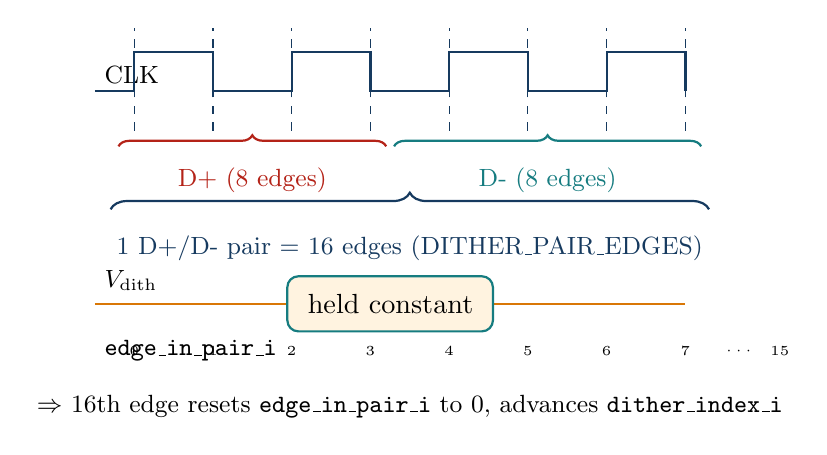
\begin{tikzpicture}[node distance=0.8cm]
% CLK waveform
\node[anchor=west] at (0,3.2) {\small CLK};
\draw[thick,navy] (0,3) -- (0.5,3) -- (0.5,3.5) -- (1.5,3.5) -- (1.5,3) -- (2.5,3) -- (2.5,3.5) -- (3.5,3.5) -- (3.5,3) -- (4.5,3) -- (4.5,3.5) -- (5.5,3.5) -- (5.5,3) -- (6.5,3) -- (6.5,3.5) -- (7.5,3.5) -- (7.5,3);
\foreach \x in {0.5,1.5,...,7.5} \draw[navy,dashed] (\x,2.5) -- (\x,3.8);

% D+ region
\draw[thick,redx,decorate,decoration={brace,amplitude=4pt}] (0.3,2.3) -- (3.7,2.3) node[midway,below=4pt,redx]{\small D+ (8 edges)};
% D- region
\draw[thick,teal,decorate,decoration={brace,amplitude=4pt}] (3.8,2.3) -- (7.7,2.3) node[midway,below=4pt,teal]{\small D- (8 edges)};
% Pair region
\draw[thick,navy,decorate,decoration={brace,amplitude=6pt}] (0.2,1.5) -- (7.8,1.5) node[midway,below=6pt,navy]{\small 1 D+/D- pair = 16 edges (DITHER\_PAIR\_EDGES)};

% Dither value
\node[anchor=west] at (0,0.6) {\small $\Vdith$};
\draw[thick,orange] (0,0.3) -- (7.5,0.3) -- (7.5,0.3);
\node[smallblock,fill=lightorange] at (3.75,0.3) {held constant};

% Edge counter
\node[anchor=west] at (0,-0.3) {\small \code{edge\_in\_pair\_i}};
\foreach \i/\x in {0/0.5,1/1.5,2/2.5,3/3.5,4/4.5,5/5.5,6/6.5,7/7.5} \node[font=\tiny] at (\x,-0.3) {\i};
\node[font=\tiny] at (8.2,-0.3) {$\cdots$};
\node[font=\tiny] at (8.7,-0.3) {15};

\node at (4,-1) {\small $\Rightarrow$ 16th edge resets \code{edge\_in\_pair\_i} to 0, advances \code{dither\_index\_i}};
\end{tikzpicture}
\caption{D+/D$-$ 对的时序结构：16 个 CLK 上升沿构成一对，抖动电压在整个对内保持不变}
\label{fig:timing}
\end{figure}

\subsection{状态机逻辑}

CLK 上升沿触发的状态机如\cref{alg:state_machine}所示。

\begin{algorithm}[H]
\caption{CLK 上升沿抖动状态机}
\label{alg:state_machine}
\begin{algorithmic}[1]
\Require \code{CAL}, \code{CAL\_DITHER\_ENABLE}, \code{DITHER\_LEVELS}, \code{DITHER\_PAIR\_EDGES}
\Ensure \code{dither\_v\_i}, \code{comp\_state\_i}
\If{\code{cal\_i} $\neq 0$ \textbf{且} \code{CAL\_DITHER\_ENABLE} $\neq 0$}
    \If{\code{edge\_in\_pair\_i} $== 0$}
        \If{\code{dither\_index\_i} $\geq$ \code{DITHER\_LEVELS}}
            \State \code{dither\_index\_i} $\gets 0$ \Comment{循环回绕}
        \EndIf
        \State $\Vdith \gets \Vlsb \cdot \left(\frac{\code{dither\_index\_i}+0.5}{N} - 0.5\right)$ \Comment{更新抖动}
        \State \code{dither\_index\_i} $\gets$ \code{dither\_index\_i} $+ 1$
    \EndIf
    \State \code{edge\_in\_pair\_i} $\gets$ \code{edge\_in\_pair\_i} $+ 1$
    \If{\code{edge\_in\_pair\_i} $\geq$ \code{DITHER\_PAIR\_EDGES}}
        \State \code{edge\_in\_pair\_i} $\gets 0$ \Comment{对结束}
    \EndIf
\Else
    \State $\Vdith \gets 0$ \Comment{正常模式：零抖动}
    \State \code{edge\_in\_pair\_i} $\gets 0$
\EndIf
\State $\vdiff \gets V(P,N) - \code{VOS} - \Vdith$
\State \code{comp\_state\_i} $\gets \begin{cases} 1 & \vdiff > 0 \\ 0 & \vdiff < 0 \\ \code{TIE\_P\_GT\_N} & \vdiff = 0 \end{cases}$
\end{algorithmic}
\end{algorithm}

\begin{keybox}{抖动更新时机}
抖动\textbf{仅在每对的第一个边沿（\code{edge\_in\_pair\_i == 0}）更新}。这意味着 D+ 的 8 次判决和 D$-$ 的 8 次判决使用\textbf{同一个抖动电压}。这是设计上的关键选择：保证 D+ 和 D$-$ 在相同阈值条件下测量，使 $R \approx D_+ - D_-$ 的残差公式有效。
\end{keybox}

\subsection{为什么 D+/D$-$ 对内保持抖动不变？}

校准引擎通过 D+/D$-$ 差分测量消除比较器固定失调。如果 D+ 和 D$-$ 使用不同的抖动电压，则：

\begin{equation}
R = D_+ - D_- = (R_{\mathrm{true}} + \Vdith^{(+)}) - (R_{\mathrm{true}} + \Vdith^{(-)}) = \Vdith^{(+)} - \Vdith^{(-)}
\end{equation}

残差将包含抖动差值，而非目标残差。因此\textbf{抖动必须在 D+/D$-$ 对内保持不变}，才能让差分测量正确抵消抖动偏置。

% ==================== 7. 比较器判决逻辑 ====================
\section{比较器判决逻辑}

\subsection{有效差分输入}

比较器的判决基于\textbf{有效差分输入}：

\begin{equation}
\boxed{
\vdiff = V(P, N) - \code{VOS} - \Vdith
}
\label{eq:vdiff}
\end{equation}

其中：
\begin{itemize}[leftmargin=2em]
    \item $V(P, N) = V_P - V_N$：物理差分输入；
    \item $\code{VOS}$：输入等效失调（默认 0）；
    \item $\Vdith$：当前抖动电压（校准模式下非零，正常模式下为零）。
\end{itemize}

\subsection{判决规则}

\begin{equation}
\code{comp\_state\_i} = \begin{cases}
1 & \text{若 } \vdiff > 0 \\
0 & \text{若 } \vdiff < 0 \\
\code{TIE\_P\_GT\_N} & \text{若 } \vdiff = 0
\end{cases}
\label{eq:decision}
\end{equation}

$\vdiff = 0$ 的精确平衡情况由 \code{TIE\_P\_GT\_N} 参数决定（默认 0，即判负）。这避免了仿真中的不确定行为。

\begin{tipbox}{抖动等效于阈值偏移}
从\cref{eq:vdiff}看，$\Vdith$ 是\textbf{从输入中减去}的，等价于将比较器判决阈值从 $V_{\mathrm{OS}}$ 移动到 $V_{\mathrm{OS}} + \Vdith$。当 $\Vdith > 0$ 时，需要更大的 $V_P - V_N$ 才能触发 COMP=1，即比较器变"迟钝"；当 $\Vdith < 0$ 时，比较器变"灵敏"。这正是"阈值抖动"的物理含义。
\end{tipbox}

% ==================== 8. CAL=0 时的零抖动路径 ====================
\section{CAL=0 时的零抖动路径}

当 \code{cal\_i == 0}（正常转换模式）时，状态机进入 else 分支：

\begin{lstlisting}[language=Verilog]
end else begin
    dither_v_i = 0.0;
    edge_in_pair_i = 0;
end
\end{lstlisting}

抖动电压被强制清零，边沿计数器也复位。这保证了：

\begin{enumerate}[leftmargin=2em]
    \item \textbf{Bypass 测试有效}：比较器在正常模式下完全理想，可用于验证 SAR 逻辑和 CDAC 的固有性能；
    \item \textbf{校准后 A/B 测试有效}：用校准权重解码 vs 用标称权重解码的对比，只反映权重的改善，不受抖动污染；
    \item \textbf{从 CAL 模式切换到正常模式的过渡干净}：只要 \code{CAL} 下降沿到来，抖动立即归零，没有残留状态。
\end{enumerate}

\begin{warnbox}{设计约束}
如果 \code{CAL=0} 时残留任何抖动（例如忘记在 else 分支清零），校准后 A/B 测试的 SNDR 对比将失去意义，因为抖动本身会引入 1-2 LSB 的码值分散。V6 通过显式的 \code{dither\_v\_i = 0.0} 和 \code{edge\_in\_pair\_i = 0} 两条语句杜绝了这一风险。
\end{warnbox}

% ==================== 9. 输出级设计 ====================
\section{输出级设计}

\subsection{有限 R 驱动}

\begin{lstlisting}[language=Verilog]
I(COMP) <+ (V(COMP) - VHIGH * transition(comp_state_i, TD, TR, TF)) / RDRV;
I(COMN) <+ (V(COMN) - VHIGH * transition(1-comp_state_i, TD, TR, TF)) / RDRV;
\end{lstlisting}

输出级采用\textbf{有限电阻电压源}模型，而非理想电压源。这是为了避免 Verilog-A 仿真中的\textbf{刚性支路环路}（rigid-branch loop）问题。

\begin{notebox}{刚性支路环路}
如果两个理想电压源直接并联（例如比较器输出驱动下一级逻辑的输入电容），Verilog-A 求解器会遇到 $0\Omega$ 环路，导致 Newton-Raphson 迭代不收敛。引入 \code{RDRV=1$\Omega$} 串联电阻后，环路电阻为有限值，保证收敛性。代价是输出高电平在驱动重负载时会略有跌落，但对于驱动数字逻辑输入（高阻）而言影响可忽略。
\end{notebox}

\subsection{transition 函数}

\code{transition(comp\_state\_i, TD, TR, TF)} 将离散状态 \code{comp\_state\_i}（0 或 1）转换为连续电压波形：

\begin{itemize}[leftmargin=2em]
    \item \code{TD=20ps}：传输延迟；
    \item \code{TR=10ps}：上升时间；
    \item \code{TF=10ps}：下降时间。
\end{itemize}

这使输出波形具有有限的边沿斜率，更接近真实比较器的行为，也便于仿真器处理。

\subsection{差分互补输出}

\code{COMP} 和 \code{COMN} 严格互补：

\begin{equation}
V_{\code{COMP}} = V_{\mathrm{HIGH}} \cdot s, \quad V_{\code{COMN}} = V_{\mathrm{HIGH}} \cdot (1-s)
\end{equation}

其中 $s = \code{comp\_state\_i} \in \{0, 1\}$。这保证了在任何时刻 $V_{\code{COMP}} + V_{\code{COMN}} = V_{\mathrm{HIGH}}$，即共模电平恒定为 $V_{\mathrm{HIGH}}/2 = 0.9\,\mathrm{V}$。

% ==================== 10. 数值例子 ====================
\section{数值例子与 sub-LSB 编码原理}

\subsection{场景设定}

假设目标权重残差 $R_{\mathrm{true}} = 0.3\,\Vlsb$（即 0.3 个校准 LSB，小于 calDAC 的 4 LSB 步长）。校准引擎对 32 个 D+/D$-$ 对进行测量，每对使用不同的抖动值。

\subsection{D+ 方向的判决}

在 D+ 方向，calDAC 设置为使差分输入比参考墙高 $R_{\mathrm{true}}$。有效差分输入为：

\begin{equation}
\vdiff_k = R_{\mathrm{true}} - V_{\mathrm{dith},k} = 0.3\,\Vlsb - V_{\mathrm{dith},k}
\end{equation}

比较器输出 1 当且仅当 $\vdiff_k > 0$，即 $V_{\mathrm{dith},k} < 0.3\,\Vlsb$。

从\cref{tab:dither_values}查表，$V_{\mathrm{dith},k} < 0.3\,\Vlsb$ 的 $k$ 值为 $0 \sim 24$（共 25 个），$V_{\mathrm{dith},k} \geq 0.3\,\Vlsb$ 的 $k$ 值为 $25 \sim 31$（共 7 个）。

\begin{equation}
D_+ = \frac{\text{判决为 1 的次数}}{N} = \frac{25}{32} = 0.78125
\end{equation}

\subsection{D$-$ 方向的判决}

在 D$-$ 方向，calDAC 设置为使差分输入比参考墙低 $R_{\mathrm{true}}$（符号反转）。有效差分输入为：

\begin{equation}
\vdiff_k = -R_{\mathrm{true}} - V_{\mathrm{dith},k} = -0.3\,\Vlsb - V_{\mathrm{dith},k}
\end{equation}

比较器输出 1 当且仅当 $\vdiff_k > 0$，即 $V_{\mathrm{dith},k} < -0.3\,\Vlsb$。

从\cref{tab:dither_values}查表，$V_{\mathrm{dith},k} < -0.3\,\Vlsb$ 的 $k$ 值为 $0 \sim 3$（共 4 个）。

\begin{equation}
D_- = \frac{4}{32} = 0.125
\end{equation}

\subsection{残差恢复}

\begin{equation}
R = D_+ - D_- = 0.78125 - 0.125 = 0.65625
\end{equation}

恢复值 $R = 0.65625$ 对应 $0.65625 / 2 = 0.328\,\Vlsb$（注意 D+/D$-$ 差分使残差被放大 2 倍），与真实值 $0.3\,\Vlsb$ 的误差为 $0.028\,\Vlsb \approx 1/36\,\Vlsb$，即约 1 LSB/32 的量化精度。

\begin{keybox}{sub-LSB 编码原理}
抖动扫描将\textbf{连续残差} $R_{\mathrm{true}} \in [-0.5, +0.5)\,\Vlsb$ 映射为\textbf{离散计数} $D_+ \in [0, N]/N$。计数 $D_+$ 是 $R_{\mathrm{true}}$ 的单调函数，其斜率为 $1/\Vlsb$（每改变 $1\,\Vlsb$，$D_+$ 变化 1）。因此 $N=32$ 次测量给出了 $\Vlsb/32 \approx 25.86\,\mu\mathrm{V}$ 的有效分辨率，远小于 calDAC 的 4 LSB 步长。
\end{keybox}

\subsection{D+/D$-$ 差分消除比较器失调}

如果比较器存在固定失调 $V_{\mathrm{OS}}$，则：

\begin{equation}
\vdiff^{(+)}_k = R_{\mathrm{true}} - V_{\mathrm{OS}} - V_{\mathrm{dith},k}, \quad \vdiff^{(-)}_k = -R_{\mathrm{true}} - V_{\mathrm{OS}} - V_{\mathrm{dith},k}
\end{equation}

对应的判决计数为：

\begin{equation}
D_+ = \Pr[\Vdith < R_{\mathrm{true}} - V_{\mathrm{OS}}], \quad D_- = \Pr[\Vdith < -R_{\mathrm{true}} - V_{\mathrm{OS}}]
\end{equation}

由于抖动序列零均值，$V_{\mathrm{OS}}$ 在两个方向上产生相同的偏移。因此：

\begin{equation}
R = D_+ - D_- \approx \frac{R_{\mathrm{true}} - V_{\mathrm{OS}}}{\Vlsb} - \frac{-R_{\mathrm{true}} - V_{\mathrm{OS}}}{\Vlsb} = \frac{2 R_{\mathrm{true}}}{\Vlsb}
\end{equation}

$V_{\mathrm{OS}}$ 在差分中被\textbf{精确消除}。这是 D+/D$-$ 双向测量的核心价值。

% ==================== 11. 与 V5 的区别 ====================
\section{与早期版本的关键区别}

\begin{table}[H]
\centering
\caption{V6 与早期版本的关键区别}
\label{tab:versions}
\small
\begin{tabularx}{\textwidth}{l X X}
\toprule
特性 & 早期版本（推测） & V6 \\
\midrule
抖动类型 & 随机噪声/伪随机 & 确定性中点均匀 \\
抖动范围 & 可能不对称 & $[-0.5, +0.5)\,\Vlsb$ 严格对称 \\
D+/D$-$ 对内抖动 & 可能变化 & 严格保持不变 \\
CAL=0 时抖动 & 可能有残留 & 严格为零 \\
抖动更新时机 & 每次 CLK 边沿 & 每对第一个边沿 \\
量化误差消除 & 一阶残留 & 中点法则消除一阶项 \\
\bottomrule
\end{tabularx}
\end{table}

% ==================== 12. 工程意义 ====================
\section{工程意义与设计启示}

\subsection{确定性 vs 随机抖动}

V6 选择\textbf{确定性抖动}而非伪随机噪声，有三个关键优势：

\begin{enumerate}[leftmargin=2em]
    \item \textbf{可重复性}：每次校准的抖动序列完全相同，仿真结果可复现，便于调试；
    \item \textbf{消除一阶量化误差}：中点法则保证 32 次测量的平均值精确等于真实期望（零偏置），而随机抖动需要足够多的样本才能收敛；
    \item \textbf{覆盖完整性}：32 个抖动值精确覆盖 $[-0.5, +0.5)\,\Vlsb$ 的全部区间，无遗漏。
\end{enumerate}

\subsection{sub-LSB 分辨率的经济性}

\begin{tipbox}{为什么不在 calDAC 上直接实现更小步长？}
calDAC 的步长受限于物理电容的单位尺寸和开关寄生。将 calDAC 步长从 4 LSB 减小到 $4/32 = 0.125$ LSB 需要将 calDAC 电容阵列扩大 32 倍，这在面积和寄生上不可接受。V6 的抖动方案用\textbf{时间换精度}：32 次测量换取 32 倍分辨率提升，无需增加任何电容面积。
\end{tipbox}

\subsection{设计约束总结}

\begin{keybox}{V6 的三个关键设计约束}
\begin{enumerate}[leftmargin=1.5em]
    \item \textbf{D+/D$-$ 对内抖动必须不变}：否则差分测量无法消除抖动偏置；
    \item \textbf{CAL=0 时抖动必须为零}：否则正常转换和 A/B 测试被污染；
    \item \textbf{抖动序列必须零均值}：否则引入系统偏置，使权重估计有偏。
\end{enumerate}
\end{keybox}

% ==================== 附录 ====================
\section*{附录 A：完整源代码}
\addcontentsline{toc}{section}{附录 A：完整源代码}

\begin{lstlisting}[language=Verilog,basicstyle=\ttfamily\scriptsize]
module COM_ideal (CLK, COMN, COMP, N, P, CAL);
    input  CLK, N, P, CAL;
    output COMN, COMP;

    electrical CLK, COMN, COMP, N, P, CAL;

    parameter real VHIGH = 1.8 from (0.0:inf);
    parameter real VTH_CLK = 0.9 from (0.0:inf);
    parameter real VTH_CAL = 0.9 from (0.0:inf);
    parameter real VOS = 0.0;
    parameter real TD = 20p from [0.0:inf);
    parameter real TR = 10p from (0.0:inf);
    parameter real TF = 10p from (0.0:inf);
    parameter real RDRV = 1.0 from (0.0:inf);
    parameter integer TIE_P_GT_N = 0 from [0:1];

    parameter integer CAL_DITHER_ENABLE = 1 from [0:1];
    parameter real CAL_LSB_V = 0.8274m from (0.0:inf);
    parameter integer DITHER_LEVELS = 32 from [2:256];
    parameter integer DITHER_PAIR_EDGES = 16 from [1:64];

    integer comp_state_i;
    integer edge_in_pair_i;
    integer dither_index_i;
    integer cal_i;

    real vdiff_i;
    real dither_v_i;

    analog begin
        cal_i = (V(CAL) > VTH_CAL) ? 1 : 0;

        @(initial_step) begin
            comp_state_i = 0;
            edge_in_pair_i = 0;
            dither_index_i = 0;
            dither_v_i = 0.0;
        end

        @(cross(V(CAL) - VTH_CAL, +1)) begin
            edge_in_pair_i = 0;
            dither_index_i = 0;
            dither_v_i = CAL_LSB_V *
                ((0.5 / (1.0*DITHER_LEVELS)) - 0.5);
        end

        @(cross(V(CAL) - VTH_CAL, -1)) begin
            edge_in_pair_i = 0;
            dither_index_i = 0;
            dither_v_i = 0.0;
        end

        @(cross(V(CLK) - VTH_CLK, +1)) begin
            if ((cal_i != 0) && (CAL_DITHER_ENABLE != 0)) begin
                if (edge_in_pair_i == 0) begin
                    if (dither_index_i >= DITHER_LEVELS)
                        dither_index_i = 0;
                    dither_v_i = CAL_LSB_V *
                        (((1.0*dither_index_i + 0.5) /
                          (1.0*DITHER_LEVELS)) - 0.5);
                    dither_index_i = dither_index_i + 1;
                end
                edge_in_pair_i = edge_in_pair_i + 1;
                if (edge_in_pair_i >= DITHER_PAIR_EDGES)
                    edge_in_pair_i = 0;
            end else begin
                dither_v_i = 0.0;
                edge_in_pair_i = 0;
            end

            vdiff_i = V(P, N) - VOS - dither_v_i;
            if (vdiff_i > 0.0)
                comp_state_i = 1;
            else if (vdiff_i < 0.0)
                comp_state_i = 0;
            else
                comp_state_i = TIE_P_GT_N;
        end

        I(COMP) <+ (V(COMP) -
            VHIGH * transition(comp_state_i, TD, TR, TF)) / RDRV;
        I(COMN) <+ (V(COMN) -
            VHIGH * transition(1-comp_state_i, TD, TR, TF)) / RDRV;
    end
endmodule
\end{lstlisting}

\end{document}
